\chapter{To define}


Upload a file and generate a pdf in with spring boot....

code quality with sonarqube


\section{Exercise}

In the exercise we implement a REST endpoint that returns a PDF file.

\begin{lstlisting}
@GetMapping(value = "/pdfreport", produces = MediaType.APPLICATION_PDF_VALUE)
public @ResponseBody byte[] createPdfReport() {

    ByteArrayInputStream bis = GeneratePdfReport.createReport();

	return bis.readAllBytes();
}
\end{lstlisting}

In the example above we assume to have a helper class GeneratePdfReport that has a method returning a ByteArrayInputStream with the data of your PDF file. We use the @ResponseBody annotation on the controller method to indicate that the object returned by the method should be marshaled directly to the HTTP response body.

For creating PDF files in Java, we'll use itextpdf: \url{https://mvnrepository.com/artifact/com.itextpdf/itextpdf}.

For creating the qr code we will use the ZXing (`Zebra Crossing') API, a popular API for QR code processing in Java. You'll need to include 2 artifacts to be able to generate QR codes.

\begin{lstlisting}
<dependency>
	<groupId>com.google.zxing</groupId>
	<artifactId>core</artifactId>
	<version>3.4.0</version>
</dependency>
<dependency>
	<groupId>com.google.zxing</groupId>
	<artifactId>javase</artifactId>
	<version>3.4.0</version>
</dependency>
\end{lstlisting}

Here is the full code for filling the name and QR code in the PDF template.

\begin{lstlisting}
package be.pxl.superhero.service.impl;

import be.pxl.superhero.api.SuperheroDTO;
import be.pxl.superhero.commons.Cipher;
import com.google.zxing.BarcodeFormat;
import com.google.zxing.WriterException;
import com.google.zxing.client.j2se.MatrixToImageWriter;
import com.google.zxing.common.BitMatrix;
import com.google.zxing.qrcode.QRCodeWriter;
import com.itextpdf.text.DocumentException;
import com.itextpdf.text.Element;
import com.itextpdf.text.Image;
import com.itextpdf.text.Phrase;
import com.itextpdf.text.pdf.ColumnText;
import com.itextpdf.text.pdf.PdfContentByte;
import com.itextpdf.text.pdf.PdfReader;
import com.itextpdf.text.pdf.PdfStamper;
import org.springframework.stereotype.Component;

import java.io.ByteArrayInputStream;
import java.io.ByteArrayOutputStream;
import java.io.IOException;
import java.net.URISyntaxException;
import java.nio.file.Path;
import java.nio.file.Paths;

@Component
public class SuperheroIdCardGenerator {

    public ByteArrayInputStream superheroIdCard(SuperheroDTO superhero) {

        ByteArrayOutputStream out = new ByteArrayOutputStream();

        try {
            Path path = 
                Paths.get(ClassLoader.getSystemResource("superheroidcard.pdf").toURI());
            PdfReader pdfReader = new PdfReader(path.toUri().toURL());
            PdfStamper pdfStamper = new PdfStamper(pdfReader, out);
            PdfContentByte canvas = pdfStamper.getOverContent(1);
            ColumnText.showTextAligned(canvas, Element.ALIGN_LEFT, new Phrase(superhero.firstName() + " " + superhero.lastName()), 200, 620, 0);
            ColumnText.showTextAligned(canvas, Element.ALIGN_LEFT, new Phrase(superhero.superheroName()), 200, 550, 0);
            byte[] qrCodeImage = getQRCodeImage(Cipher.skipALetter(superhero.superheroName()), 130, 130);
            Image qrCode = Image.getInstance(qrCodeImage);
            qrCode.setAbsolutePosition(190, 360);
            canvas.addImage(qrCode);
            pdfStamper.close();
            pdfReader.close();
        } catch (DocumentException | URISyntaxException | IOException | WriterException ex) {
            // TODO: add logging - see next chapter
            throw new PdfCreationException(ex);
        }
        return new ByteArrayInputStream(out.toByteArray());
    }

    public static byte[] getQRCodeImage(String text, int width, int height) throws WriterException, IOException {
        QRCodeWriter qrCodeWriter = new QRCodeWriter();
        BitMatrix bitMatrix = qrCodeWriter.encode(text, BarcodeFormat.QR_CODE, width, height);

        ByteArrayOutputStream pngOutputStream = new ByteArrayOutputStream();

        MatrixToImageWriter.writeToStream(bitMatrix, "PNG", pngOutputStream);
        return pngOutputStream.toByteArray();
    }
}
\end{lstlisting}

The PdfReader first opens the PDF template file. The PdfStamper is used for adding the full name, the alias and the
QR code (as an image) to the template. The newly generated PDF is returned as a ByteArrayInputStream.

\begin{oefening}

All superheroes need an id card. Your job as a developer is to create a REST endpoint where we can download a pdf with the id card.

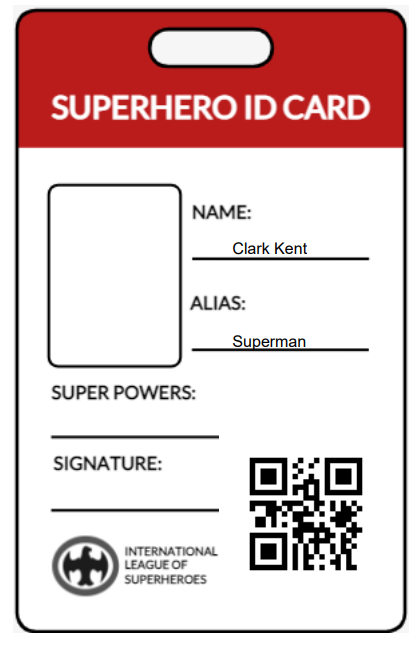
\includegraphics[width=5cm]{./images/chapter3/superhero_id_card.png}

The pdf template can be found in blackboard. 

$\square$ Download the pdf template and add it to the resources directory of your superhero-backend project.

\vspace{5mm}

We will include the full name, the superhero name and a unique QR code in the template.
The generated pdf will be available at the endpoint:
\url{http://localhost:<port>/api/superheroes/<superheroId>/idcard}

The QR code will contain the scrambled alias of a superhero. 

\vspace{5mm}

$\square$ Create the utility class Cipher with a static method skipALetter which takes a String as a parameter and returns the scrambled String. To encrypt a sentence you divide each word into half. If a word has an odd number of letters, the first group of letters contains one letter extra. Take the first letter of the first group, followed by the first letter of the second group. Then, write the second letter of the first group and the second letter of the second group, and so on, until all the words are encrypted. For example, if your sentence is `SECRET CODES', it will be encrypted as `SREECT CEOSD'.

Write unit tests to test your implementation. 
\begin{itemize}
\item unit test for one word with even length
\item unit test for one word with odd length
\item unit test for a sentence with multiple words with odd and even length
\item unit test for an empty string (should return an empty string)
\end{itemize}

\vspace{5mm}

$\square$ Implement the REST endpoint for retrieving a superhero's id card.  
\end{oefening}

\section{Code quality with SonarQube}

We would like to deliver high quality Java code. SonarQube is a Java analyzer that checks the quality of our code and detects code smells.

\begin{oefening}

Create a docker container with SonarQube. Run the following command in a terminal window:

\fbox{\strut docker run -d -{}-name sonarqube -p 9000:9000 -p 9092:9092 sonarqube}

Open \url{http://localhost:9000} in a browser. You can login with the default username `admin' and password `admin'. Next you have to update the default password (you have to choose a new password!).

\vspace{5mm}

Create a new SonarQube project for the superhero-backend application. Click on the button `Manually', fill out the project details and choose to analyze your project locally. A token will be generated.

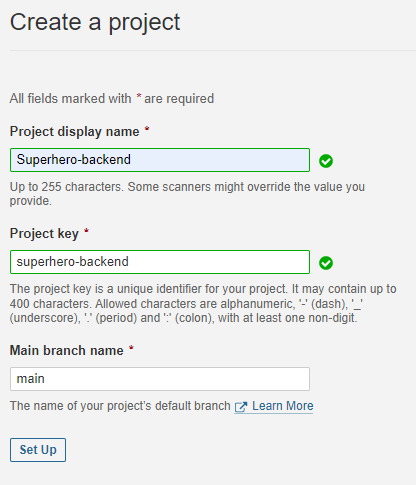
\includegraphics{./images/chapter3/sonarqube_create_project.png}

Now we can update the pom.xml file of our superhero-backend to run the code analysis.

First we need a sonar profile to provide the url, project key and token.

\begin{lstlisting}
<profiles>
	<profile>
		<id>sonar</id>
		<activation>
			<activeByDefault>true</activeByDefault>
		</activation>
		<properties>
			<sonar.host.url>http://localhost:9000</sonar.host.url>
			<sonar.projectKey>superhero-backend</sonar.projectKey>
			<sonar.login>sqp_6319ae2795ccdc24baa3a994962a8bbaa0b0cc16</sonar.login>
		</properties>
	</profile>
</profiles>
\end{lstlisting}

Run the following maven command to perform the code analysis:
\fbox{\strut \$mvn clean verify sonar:sonar}

\vspace{5mm}

Open the SonarQube dashboard \url{http://localhost:9000/dashboard?id=superhero-backend} to get an overview of possible bugs, vulnerabilities and code smells.
You can get a more in-depth explanation of the code quality rules including examples at \url{https://rules.sonarsource.com/java}. Namely, \url{https://rules.sonarsource.com/java/RSPEC-5786} is an interesting code smell to look at.

\vspace{5mm}

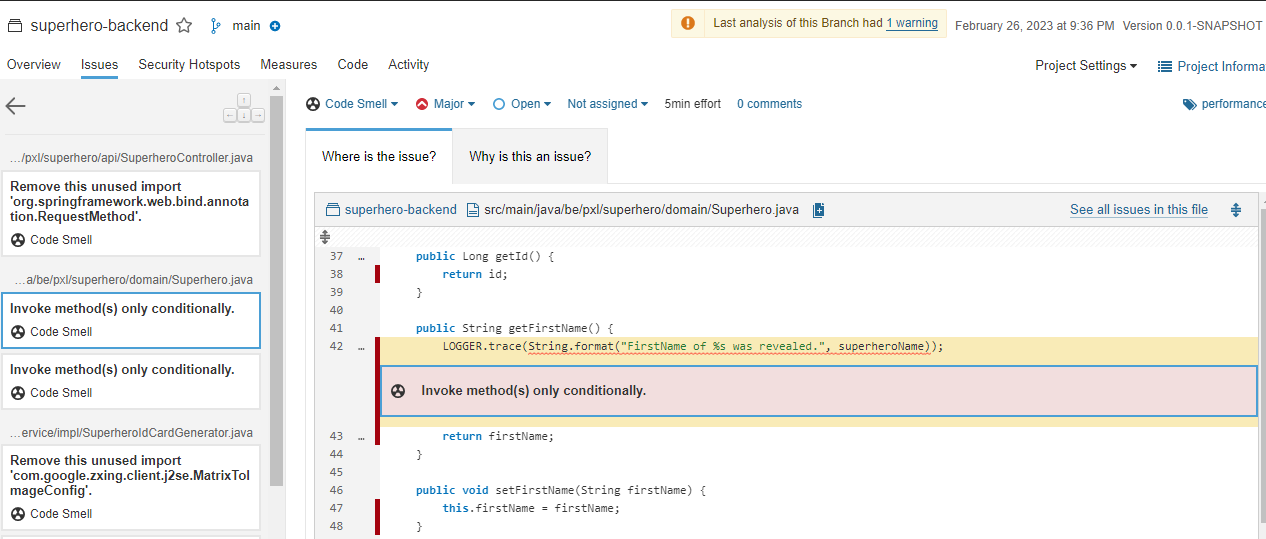
\includegraphics[width=\textwidth]{./images/chapter3/sonarqube.png}

When you look at the dashboard, you'll see the code coverage is always 0.0\%. JaCoCo is needed to generate an extra report to display the code coverage.

First add the property jacoco.version in the pom.xml file:

\begin{lstlisting}
<properties>
	<java.version>17</java.version>
	<jacoco.version>0.8.7</jacoco.version>
</properties>
\end{lstlisting}

Next, add the JaCoCo maven plugin to your project.

\begin{lstlisting}
<build>
	<plugins>
		<plugin>
			<groupId>org.jacoco</groupId>
			<artifactId>jacoco-maven-plugin</artifactId>
			<version>${jacoco.version}</version>
			<executions>
				<execution>
					<id>prepare-agent</id>
					<goals>
						<goal>prepare-agent</goal>
					</goals>
				</execution>
				<execution>
					<id>report</id>
					<phase>test</phase>
					<goals>
						<goal>report</goal>
					</goals>
				</execution>
			</executions>
		</plugin>
	</plugins>
	<pluginManagement>
		<plugins>
			...
		</plugins>
	</pluginManagement>
</build>
\end{lstlisting}

During the test phase JaCoCo will generate a report and save it in the directory target/site/jacoco/jacoco.xml. SonarQube will automatically check this location and the report will be picked up.
First remove the empty, automatically created Spring Boot test from your test folder.
Run the Maven command again and check your code coverage.

\end{oefening}

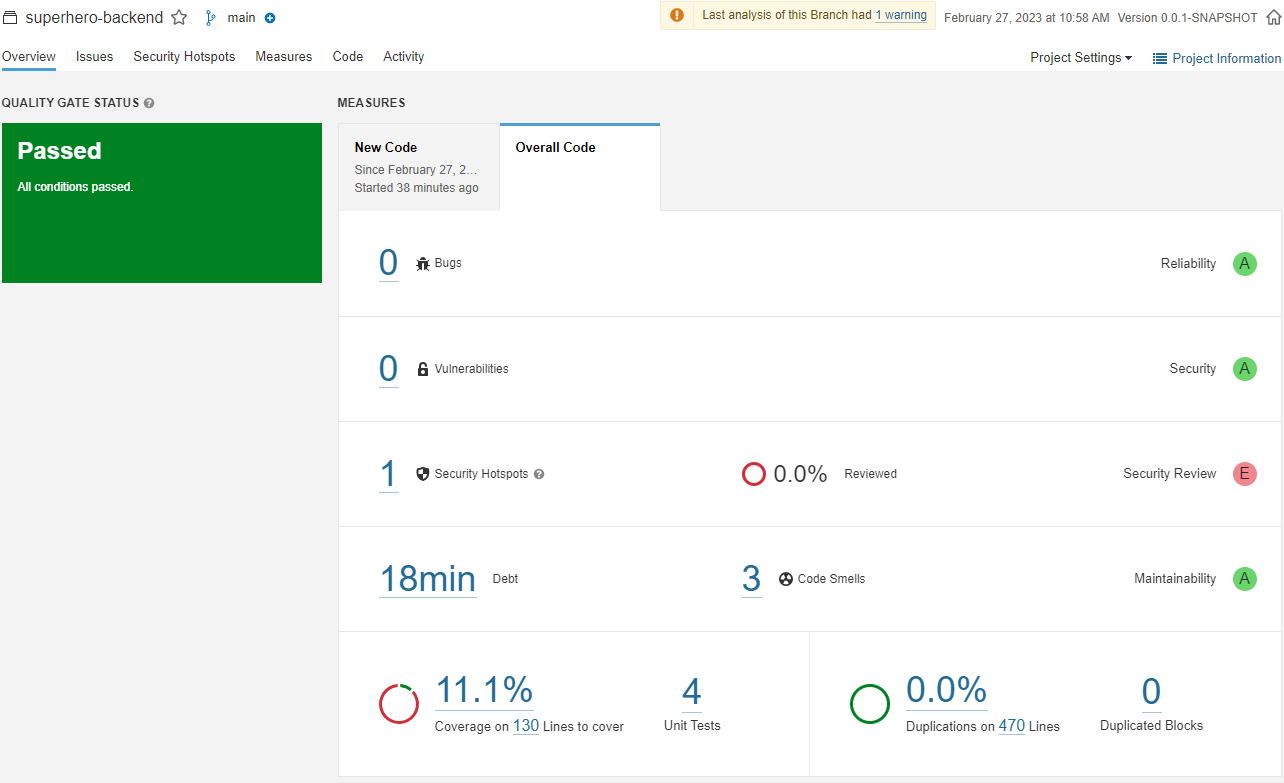
\includegraphics[width=\textwidth]{./images/chapter3/sonarqube-report.png}

A good application of priority queues is finding the shortest path in a graph. A common algorithm for this is Dijkstra’s algorithm.

https://textbooks.cs.ksu.edu/cc315/iv-priority-queues/10-heaps-and-priority-queues/5-dijkstras/